\documentclass[12pt,addpoints,answers]{exam}
\usepackage[utf8]{inputenc}
\usepackage{amsmath,amsfonts,amssymb,amsthm}
\usepackage[margin=1in]{geometry}
\usepackage{mathtools}
\usepackage{hyperref}
\usepackage{fullpage}
\usepackage{microtype}
\usepackage{xspace}
\usepackage[svgnames]{xcolor}
\usepackage[sc]{mathpazo}
\usepackage{enumitem}
\usepackage{bm}

\pagestyle{head}

%----------Header--------------------%
\def\course{{\sc Fundamentos y Aplicaciones de Blockchains}}
\def\term{Depto. de Computaci\'{o}n, UBA, 2do. Cuatrimestre 2025}
\def\prof{Lecturer: Juan Garay}
\newcommand{\handout}[5]{
   \renewcommand{\thepage}{\arabic{page}}
   \begin{center}
   \framebox{
      \vbox{
    \hbox to 5.78in { \hfill \large{\course} \hfill }
    \vspace{2mm}
%    \hbox to 5.78in { \hfill \large{\prof} \hfill }
%       \vspace{2mm}
       \hbox to 5.78in { {\Large \hfill \textbf{#5}  \hfill} }
       \vspace{2mm}
       \hbox to 5.78in { \term \hfill \emph{#2}}
       \hbox to 5.78in { {#3 \hfill \emph{#4}}}
      }
   }
   \end{center}
   \vspace*{4mm}
}
\newcommand{\hw}[4]{\handout{#1}{#2}{#3}{#4}{Homework #1}}

% -- For ignoring stuff -- %
\newcommand{\ignore}[1]{}

\begin{document}

%----Specs: change accordingly-----%
\newif\ifstudent % comment out false
\studenttrue 
% \studentfalse

\def\hwnum{1}
\def\issuedate{4/9/25}
\def\duedate{18/9/25, 17:00 hs} % 
\def\yourname{} % put your name here
%------------------------------%

\ifstudent
\hw{\hwnum}{\issuedate}{Student: \yourname}{Due: \duedate}%
\else
\hw{\hwnum}{\issuedate}{\prof}{Due: \duedate}%
\fi

% \ignore{

\noindent \textbf{Instructions}

\begin{itemize}
    \item Upload your solution to Campus; make sure it's only one file, and clearly write your name on the first page. Name the file \textsf{`$<$your last name$>$\_HW1.pdf.'} 
    %{\bf Important:} Make sure to tap {\bf Turn in} after you upload your solution.   
      
     If you are proficient with \LaTeX, you may also typeset your submission and submit in PDF format. To do so, uncomment the ``\%\textbackslash begin\{solution\}'' and ``\%\textbackslash end\{solution\}'' lines and write your solution between those two command lines.
    
      \item Your solutions will be graded on \emph{correctness} and
    \emph{clarity}. You should only submit work that you believe to be
    correct.
    % , and you will get significantly more partial credit if you     clearly identify the gap(s) in your solution.
    
    \item You may collaborate with others on this problem set.  However,
    you must \textbf{{write up your own solutions}} and \textbf{{list
      your collaborators and any external sources (including ChatGPT and similar generative AI chatbots)}} for each
    problem. Be ready to explain your solutions orally to a member of the course staff
    if asked.
    
    \ignore{
    \item For problems that require you to provide an algorithm, you must
    give a precise description of the algorithm, together with a proof
    of correctness and an analysis of its running time. You may use
    algorithms from class as subroutines. You may also use any facts
    that we proved in class or from the book.
    } %IGNORE
    
\end{itemize}

\noindent This homework contains \numquestions\ questions,
% \numpages\ pages
for a total of \numpoints \ points.
% and \numbonuspoints\ bonus points.

%\medskip
\newpage

%} %IGNORE

\begin{questions}


\question This question is about Merkle Trees (MTs).

\begin{parts}
    \part[3] Describe how (cryptographic) hash functions are used in a MT.

    \begin{solution} %Uncomment and type your solution here
        Un árbol de Merkle usa funciones hash para darle valores únicos a cada chunk.
        Dado un bloque grande de datos, lo partimos en chunks. Cada uno de esos chunks tiene
        un hash asociado. Luego, ese arreglo de hashes de cada chunk van a ser las hojas del arbol
        Las hoja número 1 y 2 van a tener un padre, que va a ser el hash de la combinacion
        de ellos mismos (es decir, de sus hashes). Lo mismo para las hojas 3 y 4, etc.

        Ahora, hacemos lo mismo para los padres de estas hojas, formando asi los abuelos de las hojas originales.
        Cada uno de estos abuelos sera padre de dos padres, combinando sus hashes. Repetimos estos pasos hasta llegar a la raíz del árbol.

        De este modo, conseguimos un identificador del árbol en muy poco espacio. Esto nos va a servir
        para las pruebas de inclusión, que nos permiten validar si el hash de un chunk que, a priori, 
        no sabemos si es el correcto. Quien quiera verificarlo tiene que reconstruir el árbol de hashes,
        asumiendo que son dados los hashes necesarios de cada bloque. Si el resultado final (la raíz) es la 
        misma que nos habíamos guardado, hemos verificado que el chunk que nos dieron era el mismo
        que teníamos antes. 

    \end{solution}

    \part[3] Describe how a (complete, binary) MT is constructed for the following five chunks of data: ABC, DEF, GHI, KLM, OPQ.

    \begin{solution} %Uncomment and type your solution here
        En este caso, al ser una cantidad de chunks impares, tenemos que decidir qué vamos a hacer.
        En mi solución, yo opté por \textbf{no duplicar los hashes del bloque impar}.

        \begin{center}
            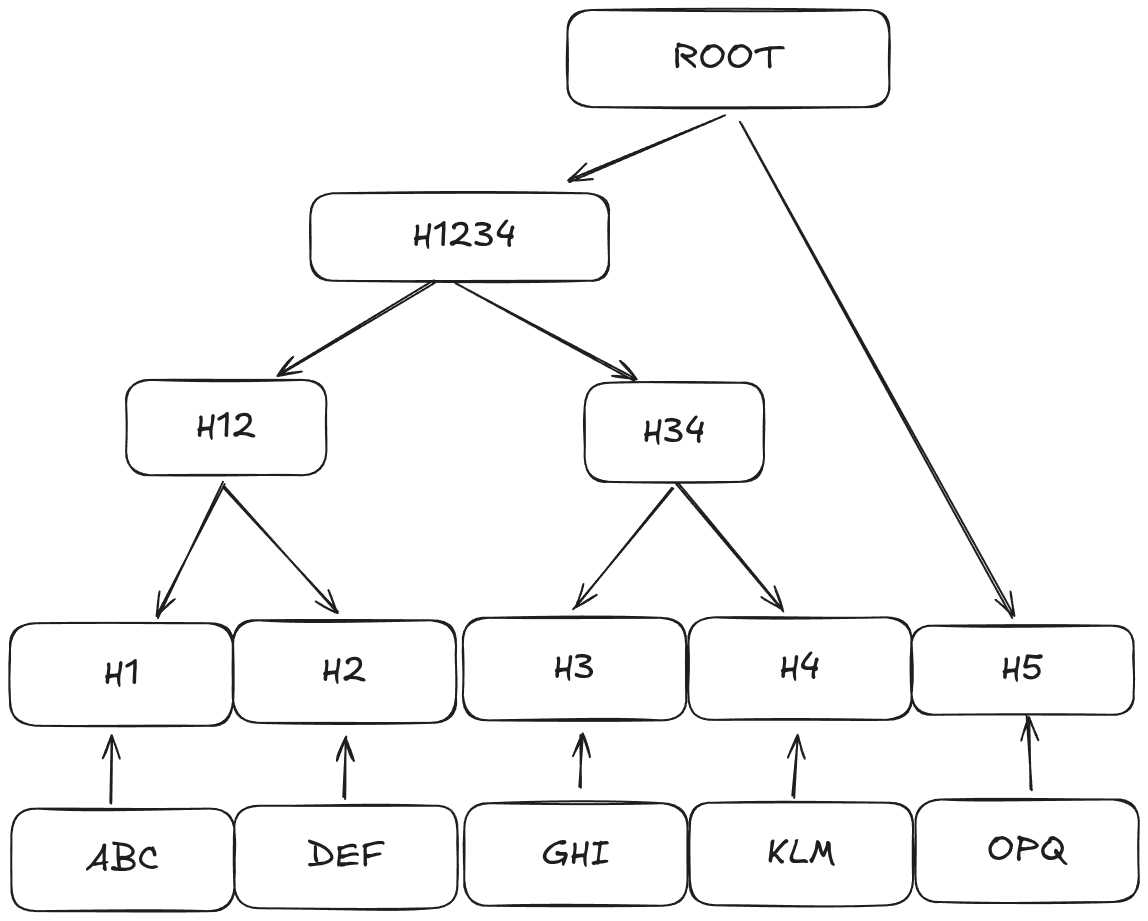
\includegraphics[width=0.62\textwidth]{ej_1_b.png}
        \end{center}
    \end{solution}
    
    \part[4] Describe how a Patricia Trie is constructed for the following key/value store: \{blah: 17, blahblah: 28, bored: 53, board: 39, aboard: 42, abroad: 17\}.

    \begin{solution}
        \begin{center}
            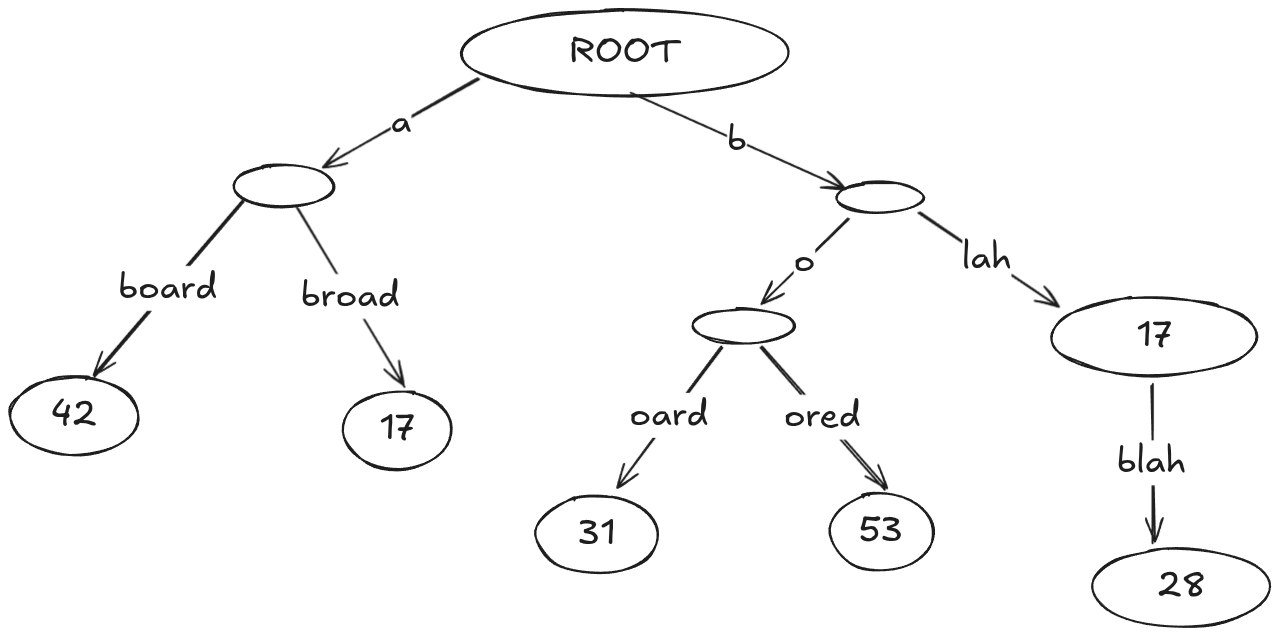
\includegraphics[width=1\textwidth]{ej_1_c.png}
        \end{center}
    \end{solution}
    
\end{parts}

\newpage

\question Cryptographic hash functions:

\begin{parts}

\part[5] Derive the formula for the {\em birthday paradox} we saw in class (show your work, explaining every step) and
calculate the number of elements needed to find a collision with at least 50\%. 

\begin{solution} %Uncomment and type your solution here
    Dado que tenemos $n$ posibles fechas y $k$ personas, la probabilidad de que dos personas tengan la misma fecha de cumpleaños es la siguiente.
    Tomamos $B$ como el evento de que todos tengan fechas de cumpleaños diferentes.
    Luego, tomar $1 - P(B)$ es la probabilidad de que haya una colisión.
   
    Notamos que la primera persona puede elegir cualquiera ($n$ posibilidades).
    
    Luego, la segunda persona puede elegir $n-1$ fechas.
    
    Y así sucesivamente.
    \begin{align*}
        P(B) &= \frac{n}{n} \cdot \frac{n-1}{n} \cdot \frac{n-2}{n} \cdot \cdots \cdot \frac{n-k+1}{n} \\
    \end{align*}

    Luego, lo que nos queda en el numerador es una permutación sin repeticiones.
    \begin{align*}
        P(B) &= \frac{n!}{(n-k)!} \cdot \frac{1}{n^k} \\
        \intertext{Ahora reescribimos la expresión anterior como un producto. Cada factor $\frac{n-i+1}{n}$ se puede reescribir como $1 - \frac{i-1}{n}$, donde $i$ va de 1 a $k$.}
        P(B) &= \prod_{i=0}^{k-1} \left(1 - \frac{i}{n}\right) \\
        \intertext{Luego, observemos que cada uno de los elementos de la productoria se ve asi $\frac{1-i}{n}$. A estos los podemos acotar superiormente por $e^{-\frac{i}{n}}$.}
        P(B) &\leq \prod_{i=0}^{k-1} e^{-\frac{i}{n}} \\
        \intertext{Luego, reescribimos la productoria como una exponencial.}
        P(B) &\leq \prod_{i=0}^{k-1} exp(-\frac{i}{n}) = exp(\frac{-1}{n} \cdot \sum_{i=1}^{k-1} i)
        \intertext{Luego, usamos la propiedad de la suma de los primeros $k-1$ enteros.}
        P(B) &\leq exp(\frac{-1}{n} \cdot \frac{(k-1)k}{2}) \\
        P(B) &\leq exp(\frac{-k(k-1)}{2n}) \\
        \intertext{Luego, despejamos $k$ a partir de $P(B) \leq exp\!\left(-\frac{k(k-1)}{2n}\right)$.}
        \ln\!\left(\frac{1}{P(B)}\right) &\geq \frac{k(k-1)}{2n} \\
        k &\geq \sqrt{2n \, \ln\!\left(\frac{1}{P(B)}\right)}
    \end{align*}
    
\end{solution}

\part[5] Apply the above result to find out how many Bitcoin users are needed to initialize their wallet’s seed, which is based on a random selection of 12 random words from the list in \url{https://github.com/bitcoin/bips/blob/master/bip-0039/english.txt}, to have the event that, with probability at least 50\%, at least two users end up with exactly the same seed.

\begin{solution} %Uncomment and type your solution here
    La idea es usar la fórmula anterior para despejar $k$ (la cantidad de usuarios).
    Vemos que esa lista tiene 2048 palabras. Si cada usuario elige 12 palabras de manera aleatoria, y 
    pueden repetirse, tenemos que $n = 2048^{12} = 2^{132}$. Para colisión con probabilidad al menos 50\%, tomamos $P(B)=0.5$.
    \begin{align*}
        k &\geq \sqrt{2n \, \ln\!\left(\tfrac{1}{P(B)}\right)} 
          = \sqrt{2 \cdot 2^{132} \, \ln 2} \\
          &\approx 8.7 \times 10^{19}
    \end{align*}
\end{solution}

\end{parts}

\newpage

\question[10] Prof. Gray has designed a cryptographic hash function $H_G : \{0, 1\}^\ast \rightarrow \{0, 1\}^n$. One of his brilliant ideas is to make $H_G(x) = x$ if $x$ is an $n$-bit string (assume the behavior of $H_G$ is much more complicated on inputs of other lengths). That way, we know with certainty that there are no collisions among $n$-bit strings. Has Prof. Gray made a good design decision? Justify your answer, in particular listing the properties that may or may not be satisfied by the design.

\begin{solution} %Uncomment and type your solution here
   La solución no es buena.
   En particular, algunas de las propiedades que \textbf{no} cumple son las siguientes:
   \begin{itemize}
    \item \textbf{Resistencia a preimagen}: Dado $y = H_G(x)$ 
    no es factible encontrar algún $x'$ tal que $H_G(x') = y$.

    En este caso (tomando que $x$ es un string de $n$ bits), si alguien conoce solamente el hash
    de un input, no es para nada difícil encontrar el input que produce ese hash.
    Se reduce a probar el mismo hash como input y se verifica la propiedad. 
    
    Siguiendo la definición que dimos, sería tomar $x' = x = y$. 
    Así se verificaría que $H_G(x') = y$.

    \item \textbf{Resistencia a segunda preimagen}: Dado $x$, no es factible encontrar
    $x' \neq x$ tal que $H_G(x) = H_G(x')$. 

    Esto tampoco lo cumple. En el caso de que $x$ \textbf{no} sea un string de $n$ bits,
    es factible encontrarlo. Tomemos $x' = H_G(x)$. Por definición de $H_G$, su codominio
    es de $n$ bits. Por lo tanto, $x' \neq x$ (pues $x$ no es de $n$ bits) y 
    vemos que $H_G(x') = H_G(H_G(x)) = H_G(x)$.

    En el caso de que $x$ sea un string de $n$ bits, es más difícil. Ahí sí tenemos que
    buscar sobre todo el espacio de los strings que no sean de $n$ bits para encontrar otro.

    \item \textbf{Pequeños cambios en el input producen grandes cambios en el output}:
    En este caso, si $x$ es un string de $n$ bits, y $x'$ es un string de $n$ bits
    que difiere en un bit, $H_G(x) \neq H_G(x')$ (es decir, no hay colisión), pero difieren solamente en un bit.
    Esto no cumple, ya que se espera que sea un cambio mayor.
    
   \end{itemize}

\end{solution}

\newpage

\question[10] As we saw in class, the main security notion for digital signatures is called {\em existential unforgeability}, which prevents an attacker from producing a signature on a message that has not been produced by the legitimate signer. I.e., the attacker should not be able to produce the pair $(m, \sigma)$, where $\sigma$ was not produced by the legitimate signer. 

Show an attack on the plain RSA signature scheme we saw in class in which an attacker forges a signature on an arbitrary message $m$ by asking the signer to sign two other different messages (not necessarily unrelated to $m$).

\begin{solution} %Uncomment and type your solution here
    Dado un mensaje arbitrario $m$, queremos mostrar como un atancante podría falsificar 
    una firma de este (llamémosla $\sigma$), pidiendole que firme dos mensajes diferentes.
    Sea $(N, e)$ la clave pública y $d$ la clave privada.

    Nuestro objetivo es construir $\sigma$ tal que $\sigma = m^d \mod N$.

    Tomemos $m_1$ y $m_2$ dos mensajes diferentes que nos pide la consigna. 
    Todavía no sabemos qué propiedad van a cumplir, pero sabemos que podemos obtener su firma.
    Luego, le pedimos al firmante que firme estos mensajes. 
    Llamamos a las firmas de estos mensajes $\sigma_1$ y $\sigma_2$. 
    Cumplen que $\sigma_1 = m_1^d \mod N$ y $\sigma_2 = m_2^d \mod N$.
    
    Volvamos a nuestro objetivo inicial. Queremos que $\sigma = m^d \mod N$.
    Qué pasa si tomamos $\sigma = \sigma_1 \cdot \sigma_2$?
    \begin{align*}
        \sigma &= \sigma_1 \cdot \sigma_2 \\
        &= (m_1^d \mod N) \cdot (m_2^d \mod N) \\
        &= (m_1 \cdot m_2)^d \mod N 
    \end{align*}

    Luego, para llegar a nuestro objetivo de $\sigma = m^d \mod N$, 
    nos basta con que $m = m_1 \cdot m_2 \mod N$

    Luego, logramos construir una firma para $m$ usando dos firmas de dos mensajes diferentes 
    entre sí (y diferentes de $m$).
   
\end{solution}

\newpage

\question[10] A Bitcoin miner creates a block $B$ which contains address $\alpha$, on which it wants to receive its rewards. An attacker changes the contents of $B$, such that instead of $\alpha$ it defines a new address $\alpha'$, which is controlled by the attacker. Will the attacker receive the rewards that the miner tries to claim? Why or why not? Give a detailed explanation of your answer.

\begin{solution} %Uncomment and type your solution here
    El problema plantea lo siguiente: un minero legítimo crea un bloque $B$ donde 
    se guarda la dirección $\alpha$, donde el minero quiere recibir sus recompensas.

    Luego, un atacante cambia el contenido de $B$, de manera que en lugar de $\alpha$, 
    define una nueva dirección $\alpha'$, controlada por él. Veamos por qué 
    el atacante no recibirá las recompensas que el minero intenta reclamar.

    El bloque en sí mismo tiene un hash asociado, que se computa 
    usando el contenido del bloque. Entonces, si el bloque cambia, el hash va a cambiar también.
    Un bloque es válido si su hash es menor que el \textit{target} actual.

    El resto de nodos (asumimos legítimos) de la red de Bitcoin, al recibir ese bloque 
    con la dirección modificada, van a computar el hash del bloque que recibieron y van a ver 
    que no cumple con la dificultad requerida (es decir, que sea menor que el \textit{target} 
    actual). Por lo tanto, el bloque no es válido.

    Si el atacante quisiera hacer que este bloque sea válido, tendría que modificar el
    \textit{nonce} del bloque, ya que el hash actual (el que incluye a $\alpha'$ como dirección) 
    no va a ser válido puesto que no va a cumplir la dificultad requerida
    (no va a ser menor que el \textit{target} actual).
        
    El rol que cumple el \textit{nonce} es de un contador que se incrementa en $1$ en cada intento
    de hash. En este intento se prueba si el hash con el nonce actual es menor que el target.
    Si es menor, el bloque es válido y se puede añadir a la cadena. Si no, se incrementa el nonce
    y se vuelve a intentar.

    Luego, para obtener un nuevo \textit{nonce} válido, el atacante tendría que hacer fuerza bruta
    hasta encontrar un \textit{nonce} que, cuando se le hace el hash a todo el bloque (proceso que
    incluye el \textit{nonce} como input de esa función hash), produzca un hash menor que el 
    \textit{target} actual.
    
    Para cuando el atacante haya encontrado un \textit{nonce} válido, la red legítima va a haber 
    avanzado con el siguiente bloque y no va a aceptar el bloque modificado por el atacante.

    De este modo concluimos que el atacante no recibirá las recompensas que el minero intenta reclamar.

\end{solution}

\newpage

\question[10] Using the course’s Sepolia  Testnet chain, send 0.05 ETH to the address of a fellow student. Describe how you conducted the payment, including the transaction’s id and addresses which you used. (Refer to the Solidity tutorial material “How to Connect
to a Public Testnet” document shared on Campus, as well as the Solidity
tutorial material and pointers.) 

\begin{solution} %Uncomment and type your solution here
   Mi dirección es {\footnotesize\texttt{0xEEE267E171c91F70C492bE8061D31aF5C5754F4c}}.

   \href{https://sepolia.etherscan.io/address/0x7F34Ef9C850b48FBD7C8c7B8EEf46C29Efc36eA4}{Esta} es la dirección del contrato que usé para enviarle 0.05 ETH a mi compañero.

   El código fuente del contrato es el siguiente:
   \begin{verbatim}
    // SPDX-License-Identifier: GPL-3.0

    pragma solidity >=0.7.0 <0.9.0;

    contract SimpleTransactionSender {
        function send(address to_address) public payable {
            payable(to_address).transfer(msg.value);
        }
    }
   
   \end{verbatim}
   Como se puede observar, es muy simple y su única función es enviar ETH a una dirección.
   Luego, usé el método \texttt{send} del contrato, con su dirección como parámetro.
   Las interacciones (al igual que el \textit{deploy}) los hice usando Remix.
   
   Finalmente, esta es la \href{https://sepolia.etherscan.io/tx/0x8151a4313435dabb1ebbf7a7f4bbb55fa69841f1d640f90ed8945c8f3d5ed42f}{transacción en Sepolia Etherscan}.

\end{solution}

\newpage
  
\question The following smart contract has been deployed on the Sepolia Testnet chain:

{\footnotesize

\begin{verbatim}
// SPDX-License-Identifier: GPL-3.0

pragma solidity >=0.7.0 <0.9.0;

contract Bank {
    mapping(address => uint256) balance;
    address[] public customers;

    event Deposit(address customer, string message);
    event Withdrawal(address customer);

    function deposit(string memory message) public payable {
        require(msg.value > 10);
        balance[msg.sender] += msg.value - 10;

        customers.push(msg.sender);

        emit Deposit(msg.sender, message);
    }

    function withdraw() public {
        uint256 b = balance[msg.sender];
        balance[msg.sender] = 0;
        payable(msg.sender).transfer(b);

        emit Withdrawal(msg.sender);
    }

    function getBalance() public view returns (uint256) {
        return balance[msg.sender];
    }
    
    function empty() public {
        require(msg.sender == customers[0]);
        
        payable(msg.sender).transfer(address(this).balance);
    }
}
\end{verbatim}

} %FOOTNOTESIZE

 Its deployed address is: {\footnotesize\texttt{0x4310a5f4Bb3b4Ff09f0694218fA50D2767a00b86}}.

 You can compile it and interact with it using Remix. You should successfully create a transaction that interacts with the contract, either depositing or withdrawing from it some coins. 
 
 \begin{parts} 
 
 \part[5] Describe the contract’s functionality (that is, the purpose of each variable, function, and event).
 
\begin{solution} %Uncomment and type your solution here
    En general, el contrato es una especie de "Banco" que permite a los usuarios depositar y retirar fondos.
    Veamos parte por parte que hace.

    \begin{itemize}
        \item \texttt{mapping}: es un diccionario que guarda, para cada dirección, el saldo de la cuenta.
        \item \texttt{customers}: es un arreglo que guarda todas las direcciones que han depositado o retirado fondos.
        \item \texttt{Deposit}: es un evento que se emite cuando un usuario deposita fondos. Además de la dirección del cliente, tiene un mensaje.
        \item \texttt{Withdrawal}: es un evento que se emite cuando un usuario retira fondos.
        \item \texttt{deposit}: es una función que permite a un usuario depositar fondos. 
        Tiene un mensaje como parámetro, que es lo que va a recibir el evento Deposit. 
        Luego, se agregan los fondos al balance de la persona que envió el dinero, restando 10 wei (por eso se requiere que se envíen mas de 10 wei).
        Algo llamativo es que se agrega la dirección del sender al arreglo de clientes, sin chequear si ya estaba ahí.

        \item \texttt{withdraw}: es una función que permite a un usuario retirar fondos. Su objetivo es vaciar el balance del que llama.
        Luego, se llama a \texttt{payable(msg.sender).transfer(b)}. Esto hace que podamos llamar a transfer para poder enviar
        el balance del usuario \texttt{b} (que es la cantidad que tenía el usuario antes de llamar a la función).
        Finalmente, se emite el evento Withdrawal con la dirección del cliente.

        \item \texttt{getBalance}: es una función que permite a un usuario ver su balance.
        \item \texttt{empty}: es una función que permite al usuario 0 vaciar todo el balance del contrato.
        Vemos que se requiere que el usuario que llama sea el primer cliente (el que está en la posición 0 del arreglo \texttt{customers}).
        Luego, se convierte la dirección del que llama a una dirección payable, para luego llamar a \texttt{transfer} para enviar
        el balance del contrato. Este balance total del contrato se obtiene con \texttt{address(this).balance}.

    \end{itemize}

\end{solution}

\part[15]
 
 Provide the id of the transaction you performed and the address you used.
 
\begin{solution} %Uncomment and type your solution here
    El id de la transacción (en la que envié 100 wei) es:
    
    {\footnotesize\texttt{0x1044bd3202eef32b72976c02c035b0992b28c6f65f1d743a1a2070902de4c493}}. 
    

    Mi dirección es {\footnotesize\texttt{0xEEE267E171c91F70C492bE8061D31aF5C5754F4c}}.

\end{solution}

\end{parts}

\newpage


\end{questions}

\end{document}
